\section{Анализ предметной области}

\begin{frame}
\frametitle{Бизнес-процессы}
\begin{figure}
    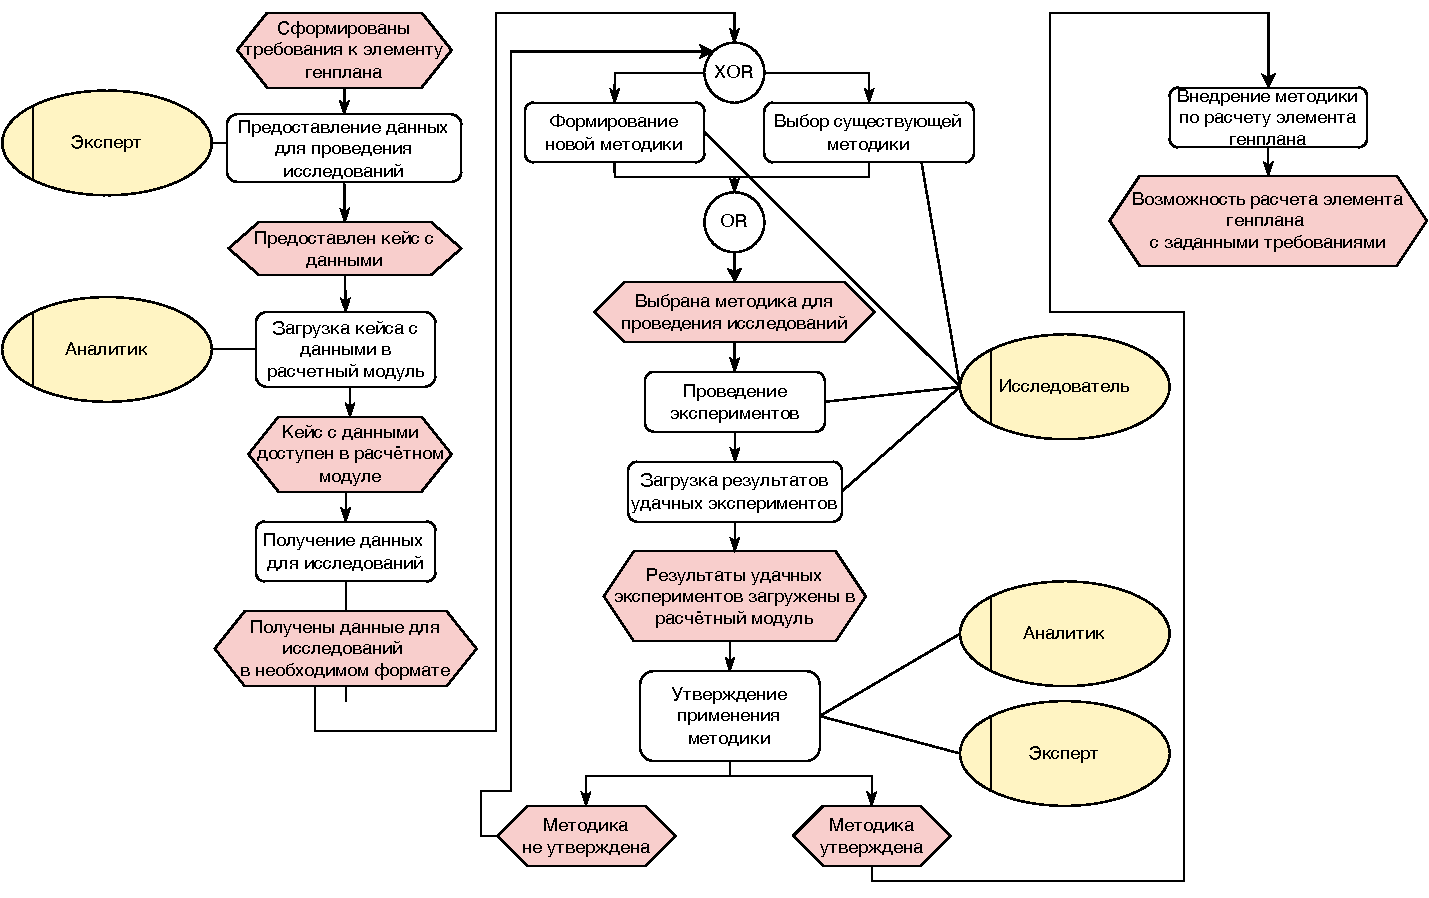
\includegraphics[scale=.48]{pictures/analysis/common_epc}
\end{figure}
\end{frame}



\section{Формирование требований}

\begin{frame}
\frametitle{Функциональные требования}
\begin{enumerate}
    \item {
        Возможность расчёта генерального плана площадного объекта в автоматическом режиме.
    }
    \item {
        Расчёт генплана должен представлять собой последовательность этапов.
    }
    \item {
        Результат каждого этапа расчёта должен быть сохранён в долговременное хранилище.
    }
    \item {
        Возможность продолжить расчёт с последнего успешно завершенного этапа.
    }
    \item {
        Возможность сравнения одинаковых расчётных объектов, полученных путем применения различных методик.
    }
    \item {
        Возможность загрузки данных, полученных от технических экспертов, в расчётный модуль.
    }
    \item {
        Возможность загрузки результатов экспериментов, а также информации об особенностях
        проведения экспериментов в расчётный модуль.
    }
\end{enumerate}
\end{frame}


\begin{frame}
\frametitle{Нефункциональные требования}
\begin{enumerate}
    \item {
        Проведение исследований на одном вычислительном сервере с операционной системой Ubuntu 20.04 LTS.
    }
    \item {
        Осуществление вызова алгоритмически сложной части системы в отдельном процессе.
    }
    \item {
        Разработанные алгоритмы должны быть оформлены в отдельную библиотеку, имеющую версионирование.
    }
    \item {
        Обеспечение высокой скорости добавления алгоритмических методик в проект.
    }
    \item {
        Обеспечение высокого уровня гибкости системы.
    }
\end{enumerate}
\end{frame}